\chapter{Deep Sentiment}

Deep Sentiment is the name of the deep neural network architecture merging both visual recognition and text analysis.

%%%%%%%%%%%%%%%%%%%%%%%%%%%%%%%%%%%%%%%%%%%%%%%%%%%%%%%%%%%%
%%%%%%%%%%%%%%%%%%%%  NEW SECTION   %%%%%%%%%%%%%%%%%%%%%%%%
%%%%%%%%%%%%%%%%%%%%%%%%%%%%%%%%%%%%%%%%%%%%%%%%%%%%%%%%%%%%
\section{The Architecture}
An illustration is worth a thousand words:

\begin{figure}[H]
    \centering
    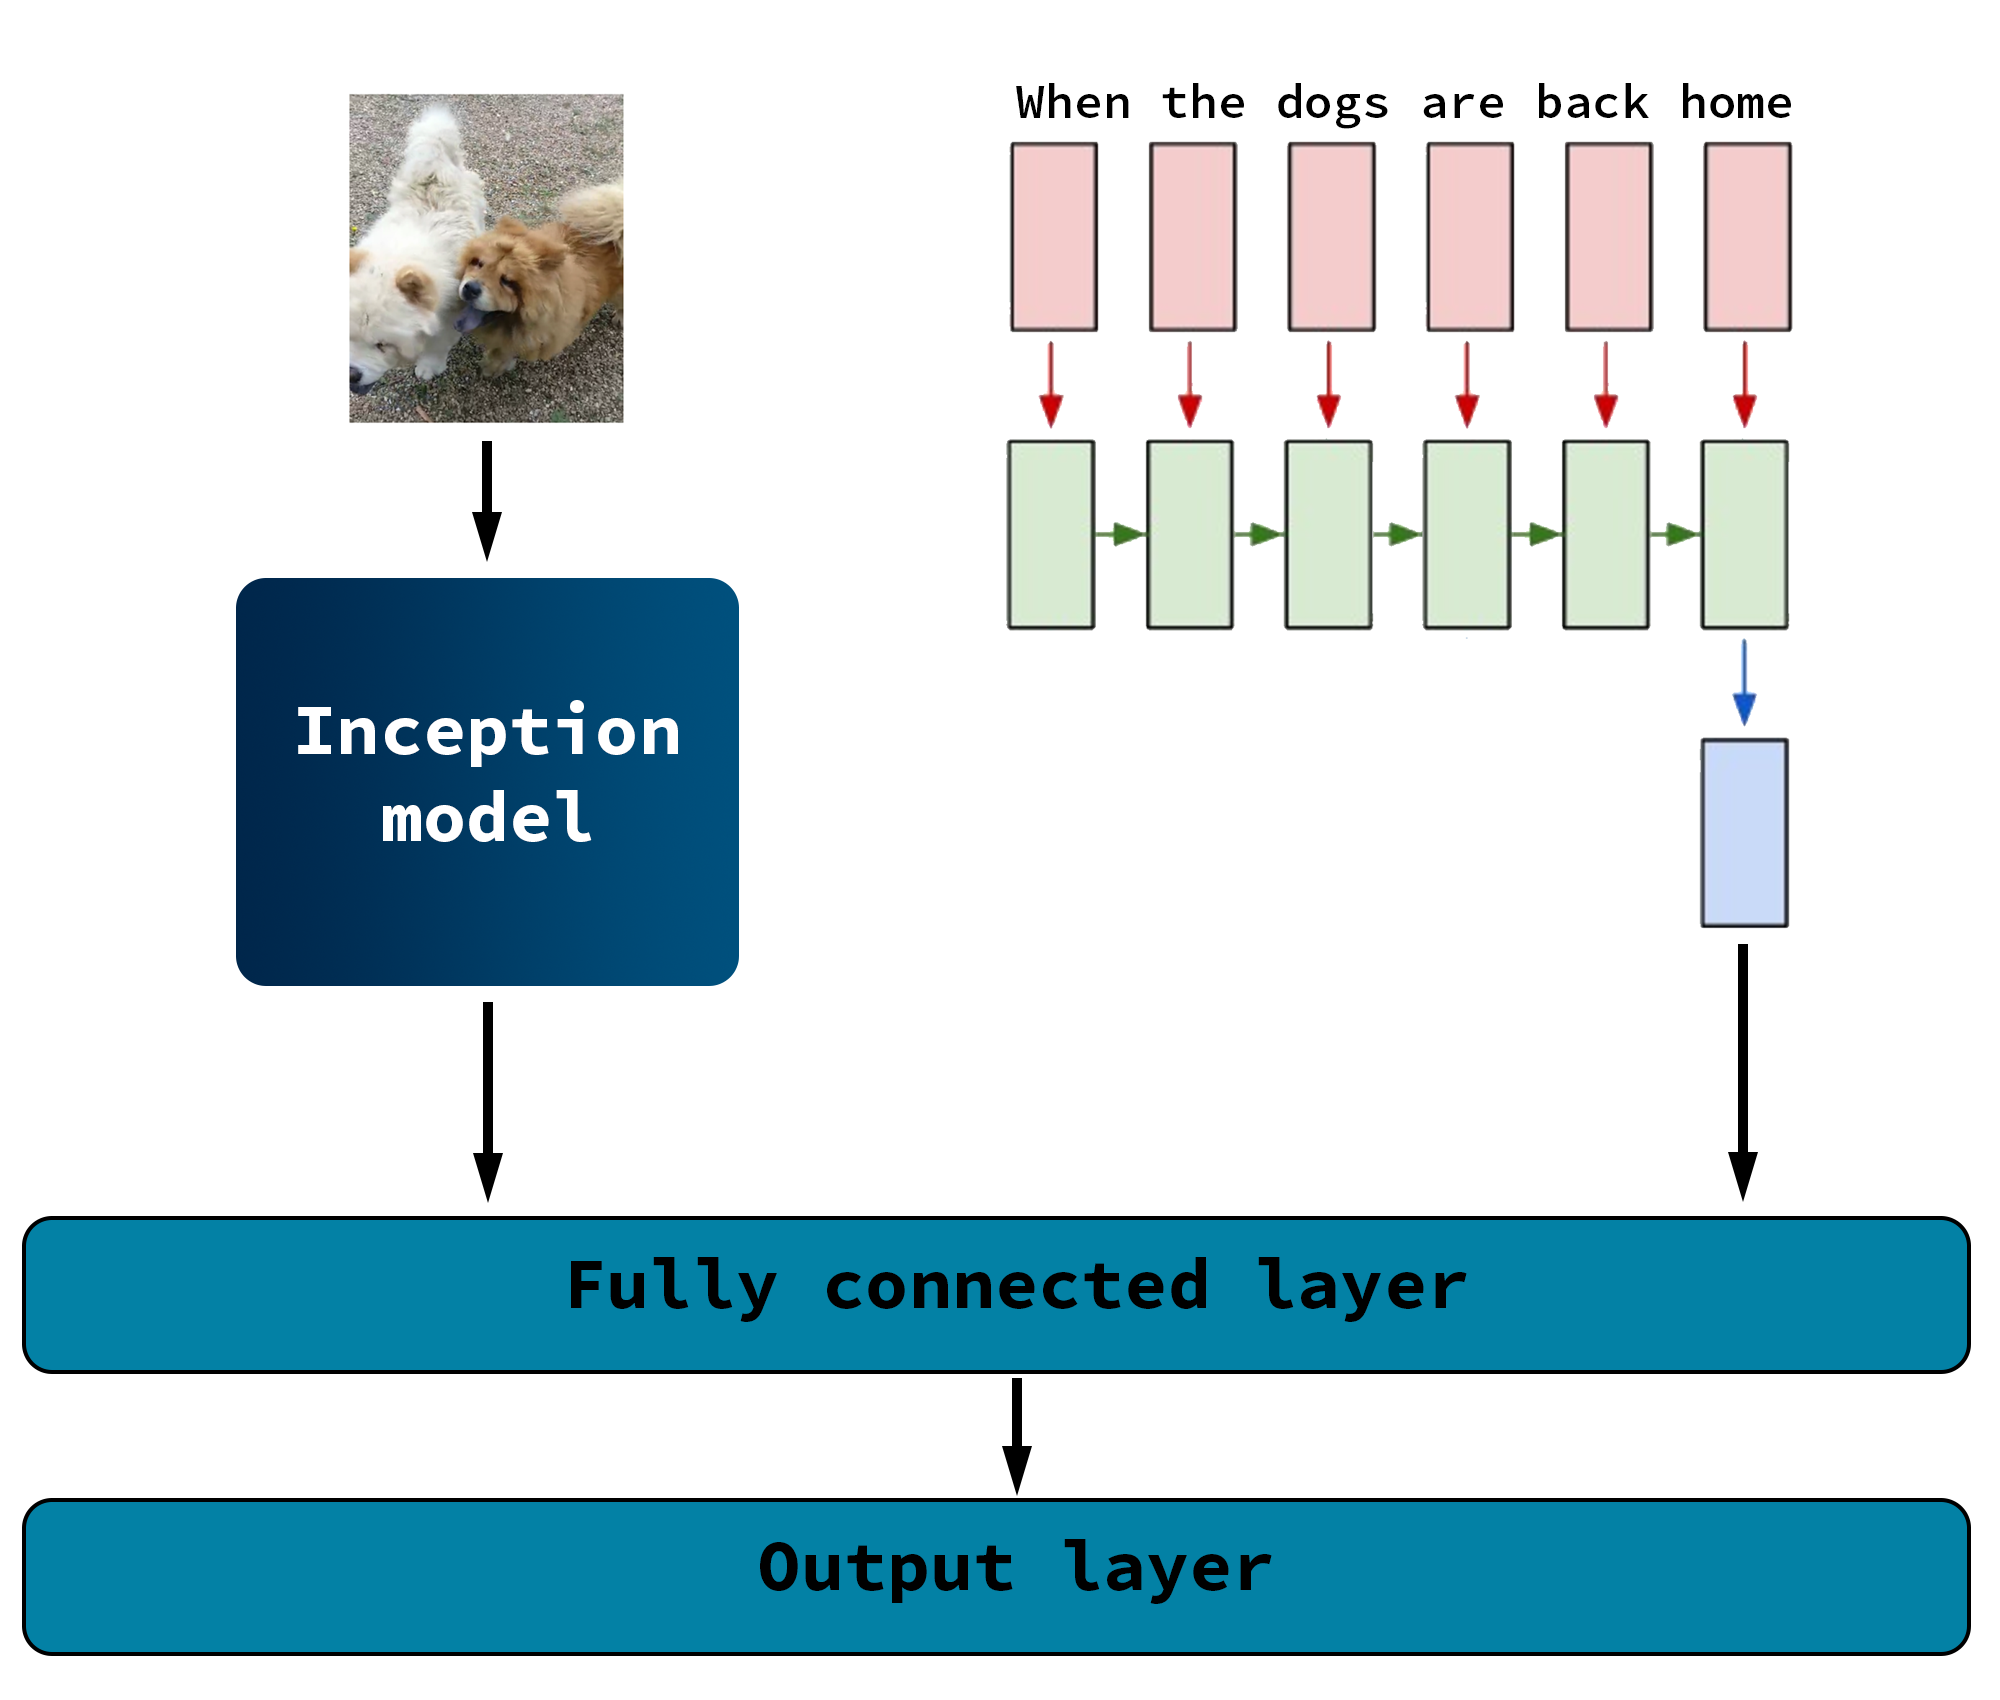
\includegraphics[width=\textwidth]{Images/deep-sentiment.png}
    \caption{Deep Sentiment architecture}
\end{figure}

\begin{enumerate}
    \item The image will go through the pre-trained Inception model that will extract features from the images.
    \item The text will be embedded in a high-dimensional space with Word2Vec and will be fed to an LSTM.
    \item The two outputs will be combined in a fully-connected layer.
    \item The final layer will give the probability distribution of the emotion of the post.
\end{enumerate}





